\documentclass[journal,12pt,twocolumn]{IEEEtran}

\usepackage{setspace}
\usepackage{gensymb} 

\singlespacing


\usepackage[cmex10]{amsmath}

\usepackage{amsthm}


\usepackage{mathrsfs}
\usepackage{txfonts}
\usepackage{stfloats}
\usepackage{bm}
\usepackage{cite}
\usepackage{cases}
\usepackage{subfig}

\usepackage{longtable}
\usepackage{multirow}

\usepackage{enumitem}
\usepackage{mathtools}
\usepackage{steinmetz}
\usepackage{tikz}
\usepackage{circuitikz}
\usepackage{verbatim}
\usepackage{tfrupee}
\usepackage[breaklinks=true]{hyperref}
\usepackage{graphicx}
\usepackage{tkz-euclide}

\usetikzlibrary{calc,math}
\usepackage{listings}
    \usepackage{color}                                            %%
    \usepackage{array}                                            %%
    \usepackage{longtable}                                        %%
    \usepackage{calc}                                             %%
    \usepackage{multirow}                                         %%
    \usepackage{hhline}                                           %%
    \usepackage{ifthen}                                           %%
    \usepackage{lscape}     
\usepackage{multicol}
\usepackage{chngcntr}

\DeclareMathOperator*{\Res}{Res}

\renewcommand\thesection{\arabic{section}}
\renewcommand\thesubsection{\thesection.\arabic{subsection}}
\renewcommand\thesubsubsection{\thesubsection.\arabic{subsubsection}}

\renewcommand\thesectiondis{\arabic{section}}
\renewcommand\thesubsectiondis{\thesectiondis.\arabic{subsection}}
\renewcommand\thesubsubsectiondis{\thesubsectiondis.\arabic{subsubsection}}


\hyphenation{op-tical net-works semi-conduc-tor}
\def\inputGnumericTable{}                                 %%

\lstset{
%language=C,
frame=single, 
breaklines=true,
columns=fullflexible
}
\begin{document}


\newtheorem{theorem}{Theorem}[section]
\newtheorem{problem}{Problem}
\newtheorem{proposition}{Proposition}[section]
\newtheorem{lemma}{Lemma}[section]
\newtheorem{corollary}[theorem]{Corollary}
\newtheorem{example}{Example}[section]
\newtheorem{definition}[problem]{Definition}

\newcommand{\BEQA}{\begin{eqnarray}}
\newcommand{\EEQA}{\end{eqnarray}}
\newcommand{\define}{\stackrel{\triangle}{=}}
\bibliographystyle{IEEEtran}
\providecommand{\mbf}{\mathbf}
\providecommand{\pr}[1]{\ensuremath{\Pr\left(#1\right)}}
\providecommand{\qfunc}[1]{\ensuremath{Q\left(#1\right)}}
\providecommand{\sbrak}[1]{\ensuremath{{}\left[#1\right]}}
\providecommand{\lsbrak}[1]{\ensuremath{{}\left[#1\right.}}
\providecommand{\rsbrak}[1]{\ensuremath{{}\left.#1\right]}}
\providecommand{\brak}[1]{\ensuremath{\left(#1\right)}}
\providecommand{\lbrak}[1]{\ensuremath{\left(#1\right.}}
\providecommand{\rbrak}[1]{\ensuremath{\left.#1\right)}}
\providecommand{\cbrak}[1]{\ensuremath{\left\{#1\right\}}}
\providecommand{\lcbrak}[1]{\ensuremath{\left\{#1\right.}}
\providecommand{\rcbrak}[1]{\ensuremath{\left.#1\right\}}}
\theoremstyle{remark}
\newtheorem{rem}{Remark}
\newcommand{\sgn}{\mathop{\mathrm{sgn}}}
\providecommand{\abs}[1]{\left\vert#1\right\vert}
\providecommand{\res}[1]{\Res\displaylimits_{#1}} 
\providecommand{\norm}[1]{\left\lVert#1\right\rVert}
%\providecommand{\norm}[1]{\lVert#1\rVert}
\providecommand{\mtx}[1]{\mathbf{#1}}
\providecommand{\mean}[1]{E\left[ #1 \right]}
\providecommand{\fourier}{\overset{\mathcal{F}}{ \rightleftharpoons}}
%\providecommand{\hilbert}{\overset{\mathcal{H}}{ \rightleftharpoons}}
\providecommand{\system}{\overset{\mathcal{H}}{ \longleftrightarrow}}
	%\newcommand{\solution}[2]{\textbf{Solution:}{#1}}
\newcommand{\solution}{\noindent \textbf{Solution: }}
\newcommand{\cosec}{\,\text{cosec}\,}
\providecommand{\dec}[2]{\ensuremath{\overset{#1}{\underset{#2}{\gtrless}}}}
\newcommand{\myvec}[1]{\ensuremath{\begin{pmatrix}#1\end{pmatrix}}}
\newcommand{\mydet}[1]{\ensuremath{\begin{vmatrix}#1\end{vmatrix}}}
\numberwithin{equation}{subsection}
\makeatletter
\@addtoreset{figure}{problem}
\makeatother
\let\StandardTheFigure\thefigure
\let\vec\mathbf
\renewcommand{\thefigure}{\theproblem}
\def\putbox#1#2#3{\makebox[0in][l]{\makebox[#1][l]{}\raisebox{\baselineskip}[0in][0in]{\raisebox{#2}[0in][0in]{#3}}}}
     \def\rightbox#1{\makebox[0in][r]{#1}}
     \def\centbox#1{\makebox[0in]{#1}}
     \def\topbox#1{\raisebox{-\baselineskip}[0in][0in]{#1}}
     \def\midbox#1{\raisebox{-0.5\baselineskip}[0in][0in]{#1}}
\vspace{3cm}
\title{ASSIGNMENT-2}
\author{C.RAMYA TULASI}
\maketitle
\newpage
\bigskip
\renewcommand{\thefigure}{\theenumi}
\renewcommand{\thetable}{\theenumi}
Download all python codes from 
\begin{lstlisting}
https://github.com/CRAMYATULASI/ASSIGNMENT-2/tree/main/ASSIGNMENT%202/CODES
\end{lstlisting}
%
and latex-tikz codes from 
%
\begin{lstlisting}
https://github.com/CRAMYATULASI/ASSIGNMENT-2/tree/main/ASSIGNMENT%202
\end{lstlisting}
%
\section{QUESTION NO-2.34}
\item Draw GOLD such that OL = 7.5, GL = 6, GD= 6, LD = 5 and OD = 10 .
%
\section{SOLUTION}
 Given,
\begin{align}
\ OL = 7.5, GL = 6, GD = 6, LD = 5, OD = 10 .
\end{align}
Now,
\begin{align}
OL=\norm{\vec{O}-\vec{L}} = 7.5
 \\
GL=\norm{\vec{G}-\vec{L}} = 6
 \\
GD=\norm{\vec{G}-\vec{D}} = 6
 \\
LD=\norm{\vec{L}-\vec{D}} = 5
 \\
OD=\norm{\vec{O}-\vec{D}} = 10
\end{align}
\begin{enumerate}
\item We know,a quadrilateral is a polygon with 4 sides if we have four points they will not form a quadrilateral if any three points are collinear. 
\item Now,let us use the above fact and consider two triangles on same base if any three points are collinear it cannot be a triangle and then given sides cannot form a quadrilateral if any three sides are collinear.
$\triangle LDO$ and $\triangle LDG$ are two triangles of given quadrilateral which are on same base $LD$ 
Now, we check if any three sides are collinear in two triangles.
Let us consider $\triangle LDO$-
\begin{align}
\norm{\vec{O}-\vec{L}}+\norm{\vec{O}-\vec{D}}&=17.5> \norm{\vec{L}-\vec{D}}\\
\norm{\vec{O}-\vec{D}}+\norm{\vec{L}-\vec{D}}&=15>\norm{\vec{O}-\vec{L}}\\
\norm{\vec{O}-\vec{L}}+\norm{\vec{L}-\vec{D}}&=12.5>\norm{\vec{O}-\vec{D}}
\end{align}
Triangle inequality is satisfied.

$\therefore$ $\triangle LDO$ can be constructed.

Similarly, Now we consider $\triangle LDG$
\begin{align}
\norm{\vec{L}-\vec{D}} + \norm{\vec{G}-\vec{L}}&=11 > \norm{\vec{G}-\vec{D}}
\\
\norm{\vec{G}-\vec{L}} + \norm{\vec{G}-\vec{D}}&=12 > \norm{\vec{L}-\vec{D}}
\\
\norm{\vec{L}-\vec{D}} + \norm{\vec{G}-\vec{D}}&=11 > \norm{\vec{G}-\vec{L}}
\end{align}
Triangle inequality is satisfied.

$\therefore$ $\triangle LDG$ can be constructed.

$\therefore$ Given sides form a quadrilateral.

Vertices of quadrilateral GOLD:

Now from $\triangle LDO$ ,the sides of $\triangle LDO$ are known Which means vertices O,L and D can be obtained using example 1.2.3

Similarly,the vertices of $\triangle LDG$ can be obtained using example 1.2.3

$\therefore$ Vertices of given Quadrilateral GOLD can be written as,
\begin{align}
\vec{L}=\myvec{0\\0},\vec{D} = \myvec{5\\0}, \vec{O}=\myvec{-1.875\\7.26},\vec{G}=\myvec{2.5\\5.5}
\end{align}
Plot of the Quadrilateral GOLD :
\numberwithin{figure}{section}
\begin{figure}[ht]
    \centering
    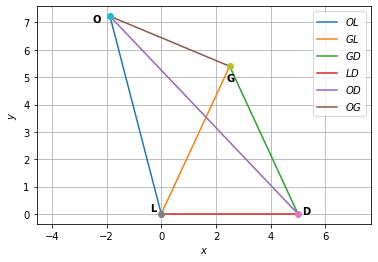
\includegraphics[width=\columnwidth]{GOLDfig.png}
    \caption{Quadrilateral GOLD}
    \label{fig:Quadrilateral GOLD}
\end{figure}
\end{enumerate}
\end{document}
